% Options for packages loaded elsewhere
\PassOptionsToPackage{unicode}{hyperref}
\PassOptionsToPackage{hyphens}{url}
%
\documentclass[
  11pt,
  oneside]{article}
\usepackage{amsmath,amssymb}
\usepackage{iftex}
\ifPDFTeX
  \usepackage[T1]{fontenc}
  \usepackage[utf8]{inputenc}
  \usepackage{textcomp} % provide euro and other symbols
\else % if luatex or xetex
  \usepackage{unicode-math} % this also loads fontspec
  \defaultfontfeatures{Scale=MatchLowercase}
  \defaultfontfeatures[\rmfamily]{Ligatures=TeX,Scale=1}
\fi
\usepackage{lmodern}
\ifPDFTeX\else
  % xetex/luatex font selection
\fi
% Use upquote if available, for straight quotes in verbatim environments
\IfFileExists{upquote.sty}{\usepackage{upquote}}{}
\IfFileExists{microtype.sty}{% use microtype if available
  \usepackage[]{microtype}
  \UseMicrotypeSet[protrusion]{basicmath} % disable protrusion for tt fonts
}{}
\makeatletter
\@ifundefined{KOMAClassName}{% if non-KOMA class
  \IfFileExists{parskip.sty}{%
    \usepackage{parskip}
  }{% else
    \setlength{\parindent}{0pt}
    \setlength{\parskip}{6pt plus 2pt minus 1pt}}
}{% if KOMA class
  \KOMAoptions{parskip=half}}
\makeatother
\usepackage{xcolor}
\usepackage[margin=1in]{geometry}
\usepackage{graphicx}
\makeatletter
\def\maxwidth{\ifdim\Gin@nat@width>\linewidth\linewidth\else\Gin@nat@width\fi}
\def\maxheight{\ifdim\Gin@nat@height>\textheight\textheight\else\Gin@nat@height\fi}
\makeatother
% Scale images if necessary, so that they will not overflow the page
% margins by default, and it is still possible to overwrite the defaults
% using explicit options in \includegraphics[width, height, ...]{}
\setkeys{Gin}{width=\maxwidth,height=\maxheight,keepaspectratio}
% Set default figure placement to htbp
\makeatletter
\def\fps@figure{htbp}
\makeatother
\setlength{\emergencystretch}{3em} % prevent overfull lines
\providecommand{\tightlist}{%
  \setlength{\itemsep}{0pt}\setlength{\parskip}{0pt}}
\setcounter{secnumdepth}{-\maxdimen} % remove section numbering
\usepackage[margin=1in]{geometry}
\ifLuaTeX
  \usepackage{selnolig}  % disable illegal ligatures
\fi
\usepackage[]{natbib}
\bibliographystyle{plainnat}
\IfFileExists{bookmark.sty}{\usepackage{bookmark}}{\usepackage{hyperref}}
\IfFileExists{xurl.sty}{\usepackage{xurl}}{} % add URL line breaks if available
\urlstyle{same}
\hypersetup{
  pdftitle={Kausalanalyse des Forschungsschwerpunkts Gesundheit des NaDiRa-Monitors},
  pdfauthor={Niklas Julius Habik (Matrikelnr.: 4726511)},
  hidelinks,
  pdfcreator={LaTeX via pandoc}}

\title{Kausalanalyse des Forschungsschwerpunkts Gesundheit des
NaDiRa-Monitors}
\usepackage{etoolbox}
\makeatletter
\providecommand{\subtitle}[1]{% add subtitle to \maketitle
  \apptocmd{\@title}{\par {\large #1 \par}}{}{}
}
\makeatother
\subtitle{Sozialwissenschaftliche Kausalanalyse (06-002-105-3)}
\author{Niklas Julius Habik (Matrikelnr.: 4726511)}
\date{2024-06-23}

\begin{document}
\maketitle

\hypertarget{einleitung}{%
\section{Einleitung}\label{einleitung}}

Prof.~Dr.~Zerrin Salikutluk war am 14.05.2024 am Insitut für Soziologie
zu Gast und referierte im Rahmen der Robert K. Merton Lecture Series
über aktuelle Forschungsergebnisse des Nationalen Diskriminierungs- und
Rassismusmonitors. Speziell wurde der Forschungsschwerpunkt Gesundheit
vorgestellt mit der konkreten Fragestellung, wie die Diskriminierung
rassistisch markierter Menschengruppen mit der Qualität der
Gesundheitsversorgung in Deutschland zusammenhängt. Zwar werden keine
Kausalhypothesen aufgestellt, doch argumentativ wird klar, welche
unterschwelligen Kausalzusammenhänge in die erhobenen Diskrimierungen
hinein interpretiert werden können.

Neben den im Forschungsbericht kommunizierten Variablen nehme ich die
Beiträge anderer Zuhörer:Innen mit in die Kausalanalyse mit auf.
Mithilfe des Programms DAGitty v3.1 versuche ich darzustellen, welche im
Vortrag und der darauffolgenden Diskussion implizierten kausalen
Argumente in das Modell eingearbeitet werden können. Ich beschreibe die
einzelnen Variablen und klassifiziere sie nach Treatments (Exposure),
Outcomes und adjustierten bzw. unbeobachteten Drittvariablen.

Am Ende der Analyse stelle ich einen potenziellen Confounder vor und
schlage eine Adjustierung vor zum prospektiven Test von
Kausalzusammenhängen. Da mir weder Frau Saliktutluks Präsentation, noch
der in naher Zukunft öffentlich publizierte Report zur Verfügung stehen,
sei angemerkt, dass es sich bei der Darstellung der Argumente und
theoretsichen Konstrukte um Rekonstruktionen eines persönlich
angefertigten erschöpfenden Protokolls des Vortrags handelt

\hypertarget{kausalanalyse}{%
\section{Kausalanalyse}\label{kausalanalyse}}

Prinzipiell folgt das Projekt der Argumentation, dass durch die von
wahrgenommener rassistischer Markierung (\textbf{\emph{RM}}) verursachte
Diskriminierung (\textbf{\emph{Disc}}) eine negative Veränderung der
Qualität der Gesundheitsversorgung (\textbf{\emph{GV}}) zur Folge hat.
Diese übt maßgeblichen Einfluss auf die Gesundheit
(\textbf{\emph{Health}}) aus. Dieser Zusammenhang steht im prinzipiellen
Forschungsinteresse und bleibt farblich im Kausaldiagramm (\emph{Figure
1}) als grüner Pfad der als gelb markierten \emph{Exposures} bis zu den
blau markierten \emph{Outcomes} nachzuvollziehen.

Erhoben wird die rassistische Markierung (\textbf{\emph{RM}}) und
Diskriminierungserfahrungen (\textbf{\emph{Disc}}) größtenteils durch
einen Selbstbericht (\textbf{\emph{Rep}}). Kontrolliert wurde auf
Unterschiede im Selbstbericht zwischen den Geschlechtern
(\textbf{\emph{Gender}}) und Ethnien (\textbf{\emph{Ethnic}}), die als
Kategorien im Selbstbericht auftauchen.

Darüber hinaus wurden experimentell Terminvergaben, ein Indikator für
die Qualität von \textbf{\emph{GV}}, experimentell erhoben und
argumentiert, dass rassistische Wissensbestände
(\textbf{\emph{RaceKnow}}) die Variation in Gesundheitsversorgungen zum
Teil erklären. Eine wichtige kausal-adjakente Variable ist der
Wissensbestand innerhalb der medizinischen Forschung
(\textbf{\emph{MedKnow}}), der durch Dokumentanalyse medizinscher
Lehrbücher und partizipatorischen Forschungsprogrammen, aber auch in
Interviews erhoben wird. Das Forschungsergebnis formuliert das Phänomen,
dass der demographische Ausgangspunkt des meisten sichergestelltem
\textbf{\emph{MedKnow}} das Ergebnis von Forschung an weißen Cis-Männern
ist.

Dem Defizit an \textbf{\emph{MedKnow}} demographischer Kontrastgruppen
wird somit als direkte Ursache für das Bestehen von unbeobachteten
\textbf{\emph{RaceKnow}} - zusammengefasst als dem als \emph{Morbus
Aliorum} bezeichneten Stigmata, dass Leiden von Personen, die vom
Ausgangspunkt des weißen Mannes askriptiv abweichen, weniger ernst
genommen werden - zusammengefasst. Untermauert wird dies beispielsweise
durch den Befund, dass muslimische Frauen tendenziell weniger
Dienstleistungen im Gesundheitssystem bekommen. Eine Darstellung
weiterer im Vortrag genannter Hinweise auf latentes
\textbf{\emph{RaceKnow}}, das sich in einem vorsätzlich durch
medizinisches Personal Qualitätsverlust der \textbf{\emph{GV}}
manifestiert, sprengt den Rahmen dieses Dokuments.

\hypertarget{analytische-korrektur}{%
\section{Analytische Korrektur}\label{analytische-korrektur}}

Hier tut sich eine erste kausale Achillessehne aus, die man bei einer
strengen Formulierung und Messung kausaler Zusammenhänge prospektiv
betrachten muss: Eine schlechtere \textbf{\emph{GV}} bestimmter Gruppen
könnte durch das Bestehen von \textbf{\emph{RaceKnow}}, also
vorsätzlicher statistischer Diskriminierung, gemutmaßt werden.
Gleichzeitig oder stattdessen könnte der Unterschied jedoch auch als
Folge des Defizits an \textbf{\emph{MedKnow}}, beispielsweise durch eine
Unterrepräsentation nicht-Weißer Ethnien in Lehrbüchern und dem
resultierenden Defizit ethnienspezifischer medizinischer Praktiken,
erklärt werden.

Personen, die beispielsweise in einer Psychotherapie keine Plätze wegen
ihrer \textbf{\emph{RM}} bekommen, können aus einer adäquaten Behandlung
ihrer psychischen Leiden ausgeschlossen werden aufgrund
\textbf{\emph{RaceKnow}} wie dem ``Morbus Aliorum'' oder dem Defizit an
\textbf{\emph{MedKnow}} wie dem vagen Forschungsstand zu psychischen
Erkrankungen subalterner Minderheiten. Sichtbar wird die
kausaltheoretische Gefahr durch die pink markierten Kausalpfade in
\emph{Figure 1.}

Eine weitere Achillessehne auf die ich aufmerksam machen möchte, ist
durch einen Diskussionbeitrag entstanden. Die Wahrnehmung der eigens
erfahrenen Diskriminierung wurde im NaDiRa kontrolliert auf
\textbf{\emph{Gender}} und \textbf{\emph{Ethnic}}. Ein aufmerksamer
Zuhörer behauptete, dass es jedoch Altersunterschiede
(\textbf{\emph{age}}) in der Wahrnehmung von Diskriminierungserfahrungen
gibt. Das ist insbesondere problematisch, wenn erwartbar ist, dass
Altersunterschiede für die Variation von \textbf{\emph{GV}}
verantwortlich sind. Auf \textbf{\emph{age}} müsste kontrolliert werden,
sollte eine potenzielle Unterschätzung des Zusammenhangs zwischen
(berichteter) Diskriminierung und verminderter \textbf{\emph{GV}}
vermieden werden.

In \emph{Figure 2} sehen wir, dass durch eine zusätzliche Kontrolle auf
\textbf{\emph{age}} und \textbf{\emph{RW}} die Pfade, die die
Kausaleffekte (\emph{Rep -\textgreater{} Disc. -\textgreater{} GV})
verzerren, geschlossen werden und eine - im Rahmen dieser Modellierung -
Kausalanalyse problemlos durchführbar wird.

\hypertarget{abbildungsverzeichnis}{%
\section{Abbildungsverzeichnis}\label{abbildungsverzeichnis}}

\begin{figure}
\centering
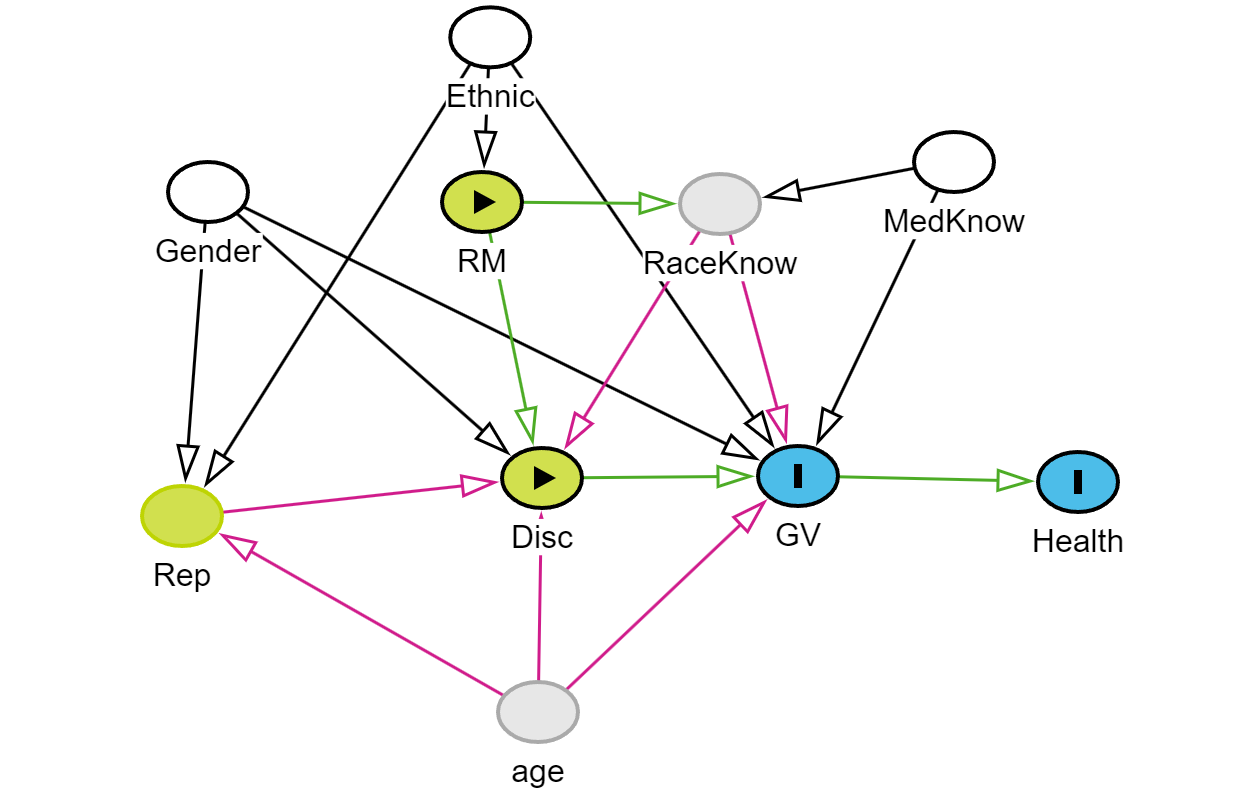
\includegraphics[width=3.125in,height=\textheight]{dagitty-model (5).png}
\caption{Empirisches Kausalmodell, erstellt in DAGitty v3.4}
\end{figure}

\begin{figure}
\centering
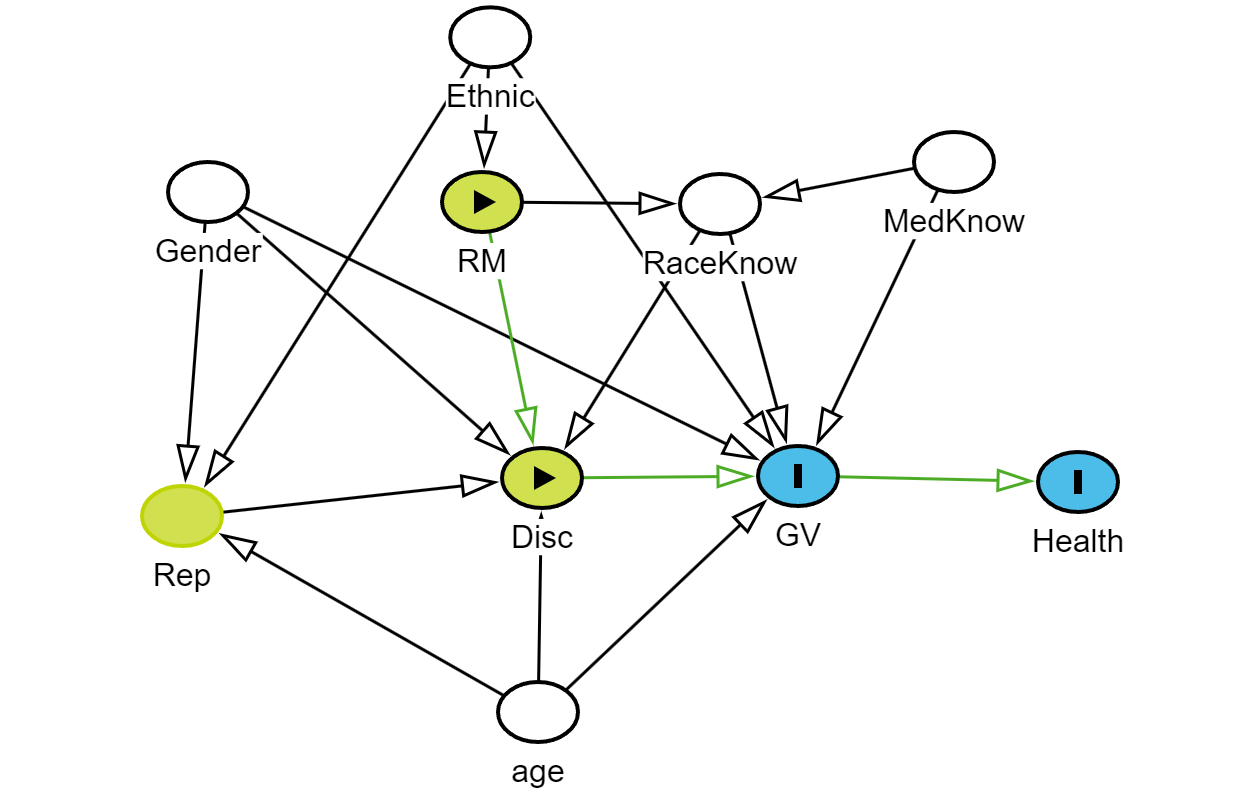
\includegraphics[width=3.125in,height=\textheight]{dagitty-model (6).png}
\caption{Modifiziertes Kausalmodell, erstellt in DAGitty v3.4}
\end{figure}

\hypertarget{glossar}{%
\section{Glossar}\label{glossar}}

RM = Rassistische Markierung\\
Disc = Diskriminierung\\
GV = Gesundheitsversorgung\\
Health = Gesundheit\\
Rep = Selbstbericht\\
Gender = Geschlecht\\
Ethnic = Ethnizität\\
RaceKnow = Rassistische Wissensbestände\\
MedKnow Medizinische Wissensbestände\\
age = Alter

  \bibliography{references.bib}

\end{document}
